\documentclass[12pt]{beamer}

\usepackage{pdfpages}
\usepackage{xeCJK}
\setCJKmainfont{STHeiti}
\setCJKsansfont{STKaiti}
\newcommand{\kaiti}{\fontfamily{STKaiti}\selectfont}
\newcommand{\heiti}{\fontfamily{STHeiti}\selectfont}

\usepackage{inputenc}
\usepackage{varwidth}
\usepackage{xcolor}
\definecolor{colora}{RGB}{214,76,71}
\definecolor{colorg}{RGB}{84,175,216}
\definecolor{colort}{RGB}{98,174,17}
\definecolor{colorc}{RGB}{253,205,103}
\definecolor{colorn}{RGB}{ 45,45,45}
\definecolor{colord}{RGB}{ 44,46,255}
\definecolor{colorb}{RGB}{ 14,41,89}
\definecolor{colori}{RGB}{255,44,45}
\definecolor{beaublue}{rgb}{0.74, 0.83, 0.9}
\definecolor{backg}{RGB}{30, 60, 150}

\usepackage{tikz}
\usetikzlibrary{arrows,shapes,backgrounds,shadows}
\tikzstyle{every picture}+=[remember picture]
\tikzstyle{na} = [baseline=-.5ex]
\tikzstyle{block} = [ultra thick, align=left, rounded corners, drop shadow, draw=black, fill=colorn,text=white]
\tikzstyle{refbg} = [rounded corners, text width=\textwidth, fill=beaublue]

\tikzstyle{blockA} = [fill=colora, draw=black, ultra thick, rounded corners, drop shadow]
\tikzstyle{blockC} = [fill=colorc, draw=black, ultra thick, rounded corners, drop shadow]
\tikzstyle{blockG} = [fill=colorg, draw=black, ultra thick, rounded corners, drop shadow]
\tikzstyle{blockT} = [fill=colort, draw=black, ultra thick, rounded corners, drop shadow]
\tikzstyle{blockN} = [fill=colorn, draw=black, ultra thick, rounded corners, drop shadow]
\tikzstyle{blockd} = [fill=colord, draw=black, ultra thick, rounded corners, drop shadow]
\tikzstyle{blockb} = [fill=colorb, draw=black, ultra thick, rounded corners, drop shadow]
\tikzstyle{blocki} = [fill=colori, draw=black, ultra thick, rounded corners, drop shadow]

\tikzstyle{circleA} = [circle, inner color = colora!20, outer color=colora, draw=black, ultra thick, rounded corners, drop shadow]
\tikzstyle{circleC} = [circle, inner color = colorc!20, outer color=colorc, draw=black, ultra thick, rounded corners, drop shadow]
\tikzstyle{circleG} = [circle, inner color = colorg!20, outer color=colorg, draw=black, ultra thick, rounded corners, drop shadow]
\tikzstyle{circleT} = [circle, inner color = colort!20, outer color=colort, draw=black, ultra thick, rounded corners, drop shadow]
\tikzstyle{circleN} = [circle, inner color = colorn!20, outer color=colorn, draw=black, ultra thick, rounded corners, drop shadow]
\tikzstyle{circled} = [circle, inner color = colord!20, outer color=colord, draw=black, ultra thick, rounded corners, drop shadow]
\tikzstyle{circleb} = [circle, inner color = colorb!20, outer color=colorb, draw=black, ultra thick, rounded corners, drop shadow]
\tikzstyle{circlei} = [circle, inner color = colori!20, outer color=colori, draw=black, ultra thick, rounded corners, drop shadow]

\pgfmathdeclarerandomlist{randomColors}{
  {colora}
  {colorc}
  {colorg}
  {colort}
}

\pgfmathdeclarerandomlist{randomBlocks}{
  {blockA}
  {blockC}
  {blockG}
  {blockT}
}

\usepackage{tcolorbox}

%\setbeamertemplate{sections in toc}[circle]
\usetheme{Frankfurt}
\usecolortheme[named=backg]{structure}
\setbeamertemplate{sections/subsections in toc}[circle]
\setbeamertemplate{itemize items}[triangle]

\setbeamertemplate{footline}{

\includegraphics[height=1.5em]{figures/copyright.png}
    \hfill
    \insertframenumber
    /
    \inserttotalframenumber
    \hspace{0.1cm}
}



\title{\huge{全基因组与目标区域DNA重测序数据分析}}
\author{\large{石\ 泉}\\shiquan@genomics.cn\\https://github.com/shiquan}
\institute{\large{华大基因研究院}}
\date{}
\begin{document}
\frame{\titlepage}
\begin{frame}{前言}
  \kaiti{本文档为华大学院组织培训《全基因组与目标区域重测序数据
      分析》课程授课课件与相关学习文档。参考文献见各页面底部,
      请点击进去。转载请注明出处。为了保证学习讨论效果,进入本课程
      学习讨论前,请先复习以下内容。}
 \begin{columns}
 \begin{column}{0.35\textwidth}
 \begin{itemize}
 \item 生物基础 \tikz \coordinate (l-i1);
 \item 测序原理 \tikz \coordinate (l-i2);
 \item Linux\\操作基础 \tikz \coordinate (l-i3);
 \end{itemize}
 \end{column}
 \begin{column}{0.65\textwidth}
 \begin{itemize}
\item \tikz \coordinate (r-i1); 中心法则(center dogma)
\item \tikz \coordinate (r-i2); DNA packaging 
\item \tikz \coordinate (r-i3); cDNA, noncoding RNA 
\item \tikz \coordinate (r-i4); 读长(reads),接头(adaptor) 
\item \tikz \coordinate (r-i5); barcoding 
\item \tikz \coordinate (r-i6); 解压压缩包 
\item \tikz \coordinate (r-i7); GNU Make,GCC 
 \end{itemize}
 \end{column}
 \end{columns}
 \begin{tikzpicture}[overlay]
 \path[->,colora,ultra thick] (l-i1) edge [in=180, out=0] (r-i1);
 \path[->,colora,ultra thick] (l-i1) edge [in=180, out=0] (r-i2);
 \path[->,colora,ultra thick] (l-i1) edge [in=180, out=0] (r-i3);
 \path[->,colorc,ultra thick] (l-i2) edge [in=180, out=0] (r-i4);
 \path[->,colorc,ultra thick] (l-i2) edge [in=180, out=0] (r-i5);
 \path[->,colorn,ultra thick] (l-i3) edge [in=180, out=0] (r-i6);
 \path[->,colorn,ultra thick] (l-i3) edge [in=180, out=0] (r-i7);
 \end{tikzpicture}
 \end{frame}

\begin{frame}
 \tableofcontents
 \end{frame}

\section{什么是DNA重测序?}
\begin{frame}\frametitle{什么是DNA''重''测序?}
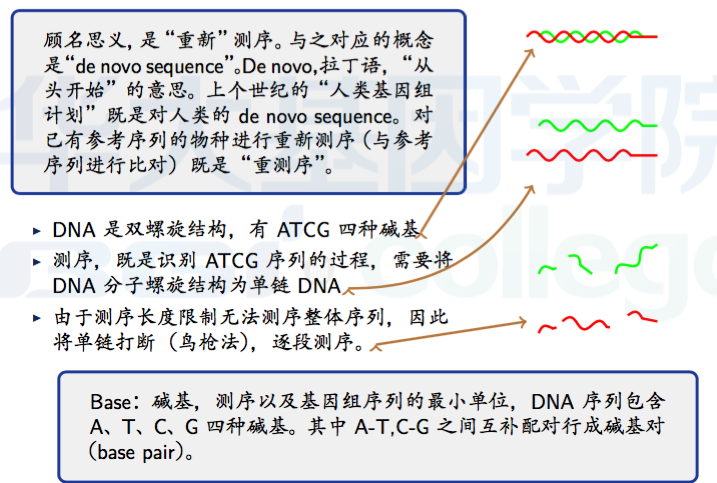
\includegraphics[width=\textwidth]{figures/old_slides/reseq.png}
\end{frame}


\section{为什么进行重测序?}
\begin{frame}\frametitle{为什么进行DNA重测序?}
  \begin{columns}
    \begin{column}{0.5\textwidth}
      \begin{itemize}
      \item 环境因素和遗传因素作用导致疾病。
      \item 器质性病变无法逆转(大叶性肺炎除外)。
      \item 蛋白测序、RNA测序难度远高于DNA测序。
      \item DNA检测的优势和适用。
      \item 早发现,早治疗。未病先防。        
      \end{itemize}
      \end{column}
    \begin{column}{0.5\textwidth}
      \includegraphics[width=\textwidth]{figures/bio_layer.pdf}
      \end{column}
    \end{columns}
  \end{frame}

\begin{frame}\frametitle{研究遗传性状(表型)的一般步骤}
  \end{frame}

\begin{frame}\frametitle{遗传变异基础}
  根据变异范围划分:
  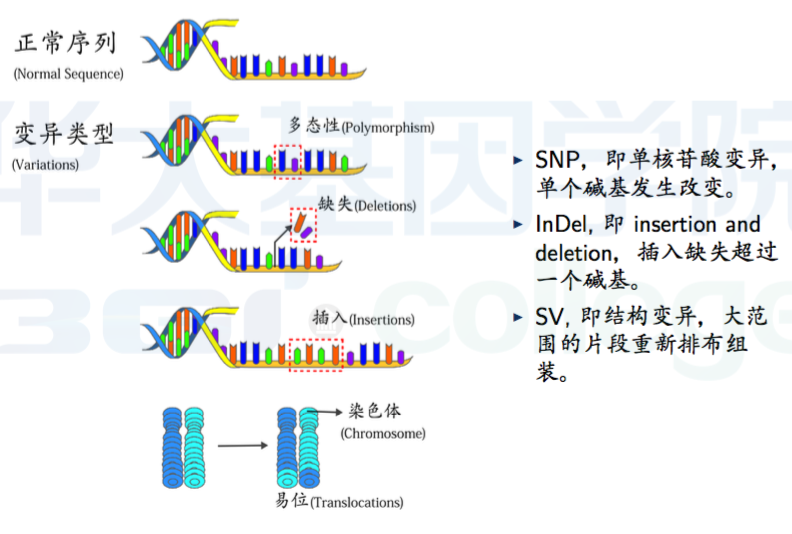
\includegraphics[width=\textwidth]{figures/old_slides/varbasic.png}
\end{frame}

\begin{frame}\frametitle{Germline and somatic (driver) mutations}
    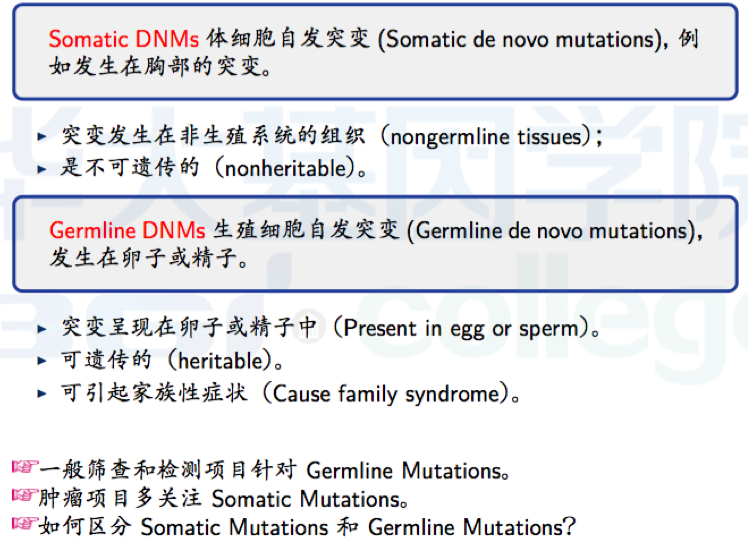
\includegraphics[width=\textwidth]{figures/old_slides/vartype.png}
  \end{frame}


\begin{frame}%\frametitle{SNV}
  \begin{center}
    {  \large  SNVs = SNPs + Point mutations}
  \end{center}
  {\small
\begin{tcolorbox}[colback=backg!5,colframe=backg,title=SNV]
  SNV 单核苷酸变异 (Single Nucleotide Variation), a single base insertion or deletion, a transition or transversion. Includes the set of SNPs.
\end{tcolorbox}
\begin{tcolorbox}[colback=backg!5,colframe=backg,title=SNP]
  SNP单核苷酸多态性(Single Nucleotide Polymorphism),指的是DNA序列上发生的单个核苷酸碱基之间的变异。在人群中这种编译的发生频率至少大于1\%,否则被认为是点突变。“在人类遗传基因的各种差异,有90\%都可归因于SNP所引起的基因变异。在人基因组中,每隔100至300个碱基就会存在一处SNP。每3个SNP中有两个会是胞嘧啶(C)和胸腺嘧啶(T)的相互转变。”
  \end{tcolorbox}
  }

\end{frame}

\begin{frame}
  \begin{tcolorbox}[colback=backg!5,colframe=backg,title=Point mutations]
   Point Mutation 点突变,是突变的一种类型,会使单一个碱基核 苷酸替换成另一种核苷酸,一般也包括只有作用于单一剪辑对 的插入或者缺失。在人群的发生率小于 1\%,与之相对的定义是 SNP(见上一页)。
  \end{tcolorbox}
  突变可依发生位置对基因功能的影响而作以下分类:
  \begin{itemize}
  \item 无义突变 (nonsense mutation),使原本可编码蛋白的密码子变成终止密码。
  \item 错义突变 (missense mutation),使密码子对应的编码氨基酸发生改变。
  \item 沉默突变 (silent mutation),密码子改变,但编码氨基酸不变。
  \end{itemize}
\end{frame}

\begin{frame}\frametitle{Insert and Deletion}
  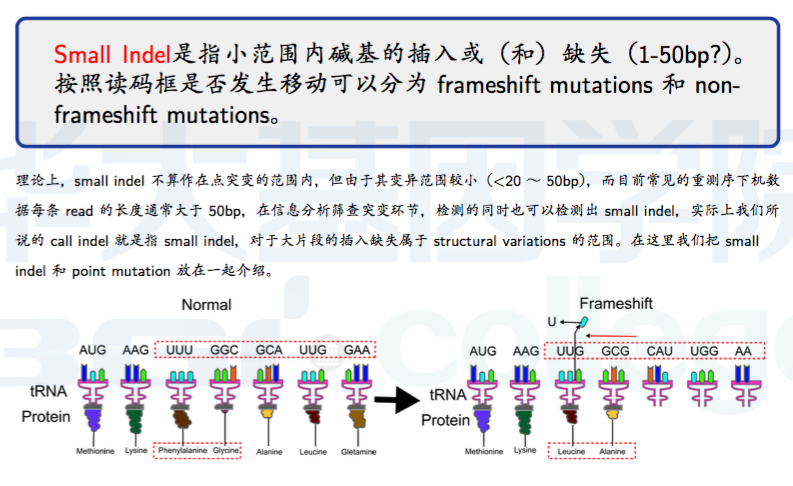
\includegraphics[width=\textwidth]{figures/old_slides/indel.png}
\end{frame}

\begin{frame}\frametitle{Splice sites}
  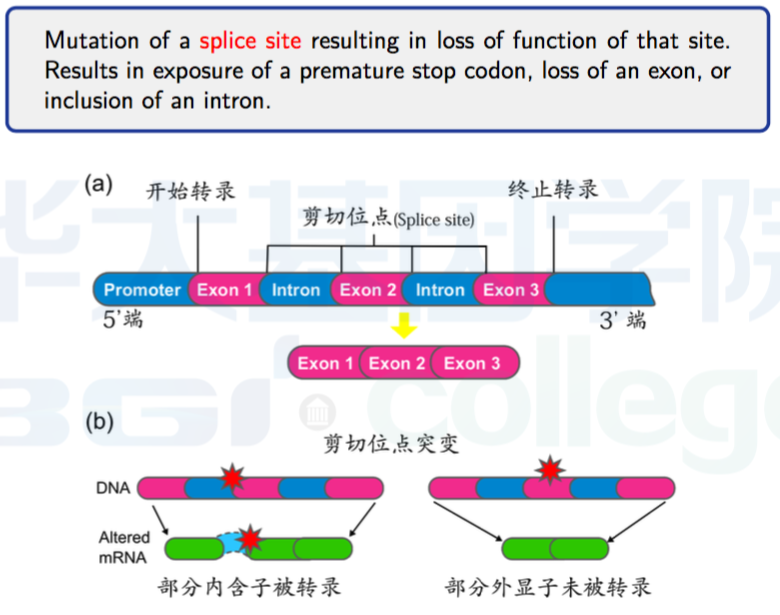
\includegraphics[width=\textwidth]{figures/old_slides/splice.png}
\end{frame}

\begin{frame}\frametitle{SV}

\end{frame}

\begin{frame}\frametitle{CNV}
  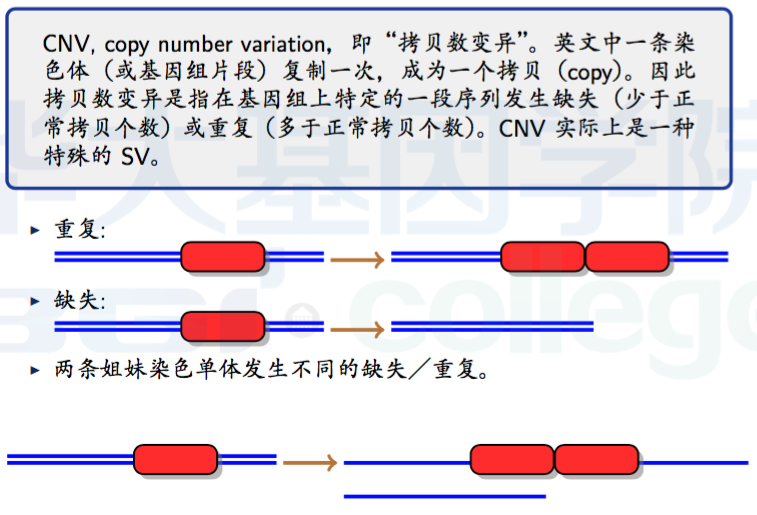
\includegraphics[width=\textwidth]{figures/old_slides/cnv.png}
\end{frame}


\section{如何进行重测序?}
\begin{frame}\frametitle{如何进行重测序?}
  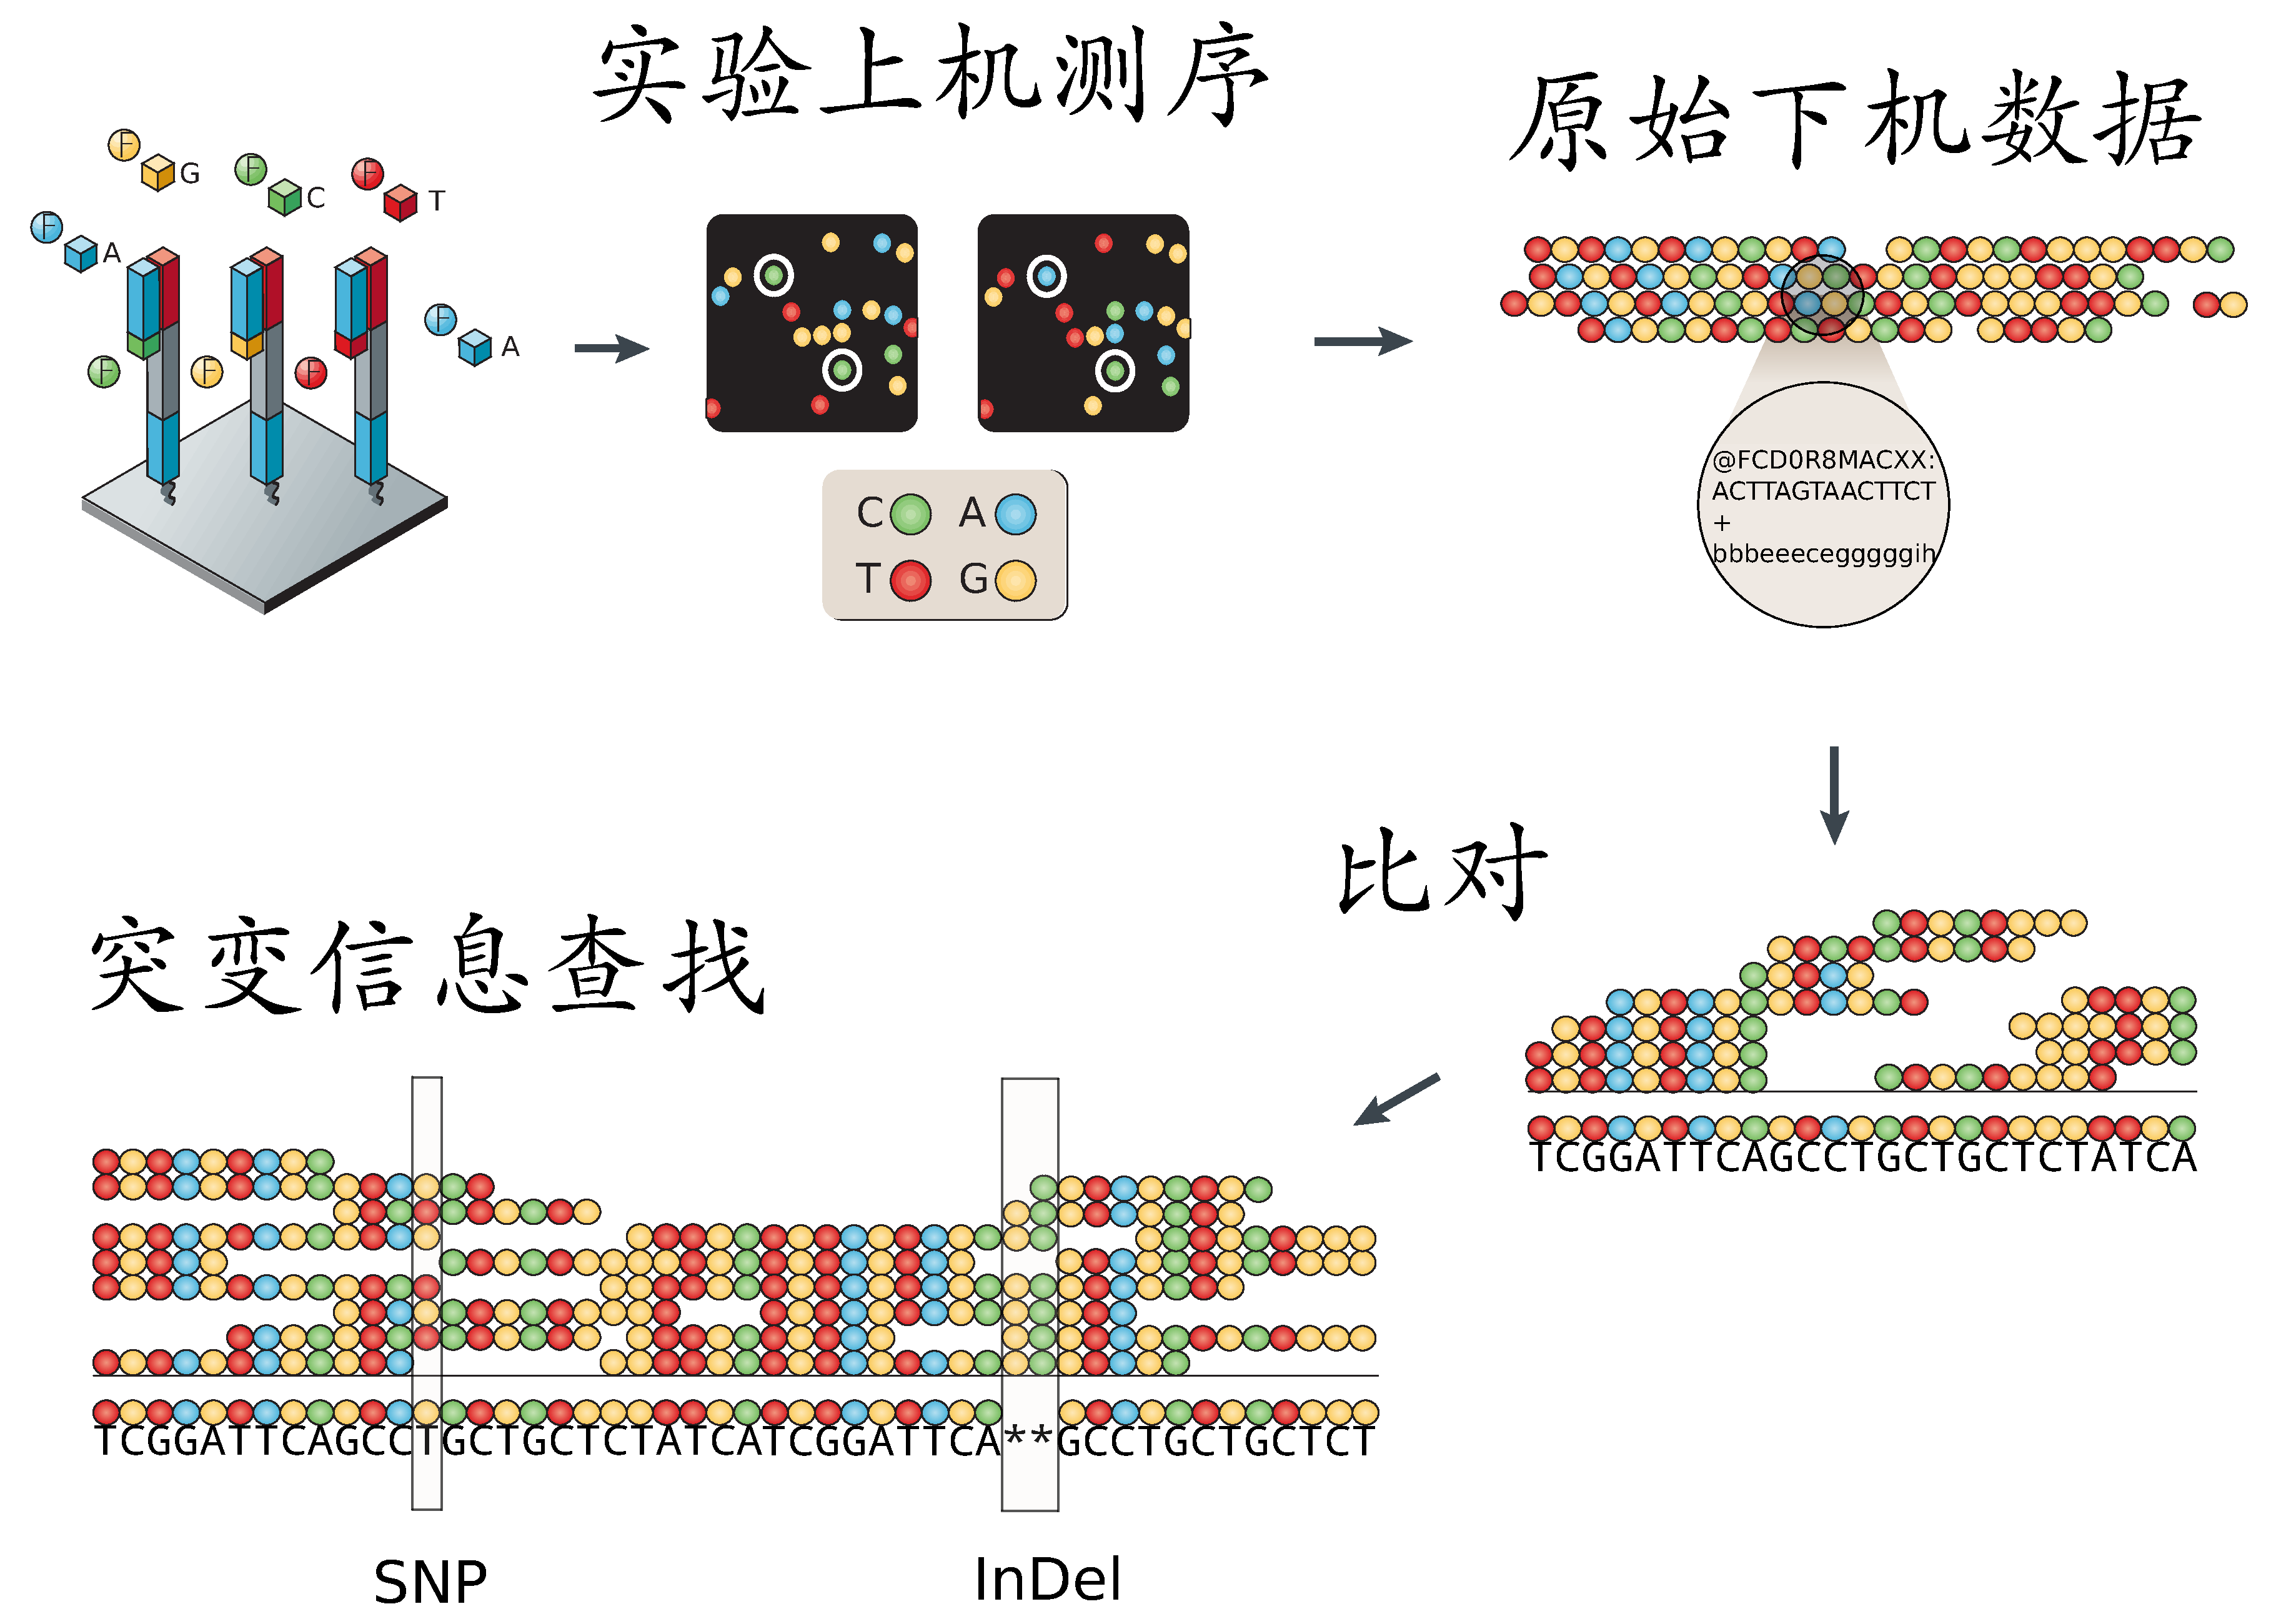
\includegraphics[width=\textwidth]{figures/reseq-pip.png}
\end{frame}

\begin{frame}
  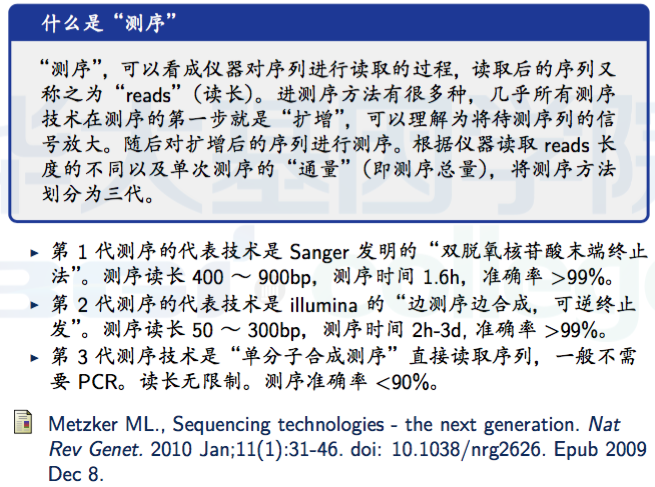
\includegraphics[width=\textwidth]{figures/old_slides/seq.png}
\end{frame}

\begin{frame}\frametitle{建库和测序方法}
\end{frame}

\begin{frame}\frametitle{插入片段(Insertsize)}
  \begin{block}{插入片段长短对信息分析的影响}
    \begin{itemize}
    \item 插入片段相对过度:接头污染(案例:酶切建库)。
    \item 插入片段长度不一(讨论)。
      \end{itemize}
    \end{block}
\end{frame}

\begin{frame}\frametitle{接头污染(Adaptor pollution)}

\end{frame}



\begin{frame}\frametitle{常规重测序分析流程(最简版)}
\end{frame}

\begin{frame}\frametitle{比对}
  {\large{\ttfamily{``The most important first step in understanding next-generation sequencing data is the initial alignment or assembly that determines whether an experiment has succeeded and provides a first glimpse into the results.''\cite{ref2}}}}



  \tikz \node[refbg]{
\begin{thebibliography}{1}
  {\small{\bibitem[Paul F., Ewan B.]{ref2}  Paul Flicek, Ewan Birney. Sense from sequence reads: methods for alignment and assembly. \emph{Nature Methods}, \textbf{Vol 6},  online: 6 May 2010.}}
\end{thebibliography}
};
\end{frame}
\begin{frame}
  
\end{frame}
\begin{frame}\frametitle{比对策略}
\end{frame}

\begin{frame}\frametitle{比对格式}
\end{frame}

\begin{frame}\frametitle{变异检测}
\end{frame}

\begin{frame}\frametitle{变异格式}
\end{frame}

\begin{frame}\frametitle{重测序分析流程(升级版1.0)}
\end{frame}

\begin{frame}\frametitle{质量控制}
\end{frame}

\begin{frame}\frametitle{深度覆盖度统计}
\end{frame}

\begin{frame}\frametitle{重测序分析流程(多样品版)}
\end{frame}

\begin{frame}\frametitle{Burden test}
\end{frame}

\begin{frame}\frametitle{重测序分析流程(非人版)}
\end{frame}

\section{为什么重测序的工作中也需要组装技术?}
\begin{frame}\frametitle{为什么重测序的工作中也需要组装技术?}
  \begin{tikzpicture}
    
  \end{tikzpicture}
\end{frame}
\begin{frame}\frametitle{组装技术}
\end{frame}

\begin{frame}\frametitle{常见组装软件}
\end{frame}

\section{测序分析流程回顾}

\begin{frame}\frametitle{测序分析流程回顾}
\end{frame}

\section{变异注释}
\begin{frame}\frametitle{变异注释}
\end{frame}
\begin{frame}\frametitle{ENCODE}
\end{frame}

\section{案例分享}
\begin{frame}\frametitle{案例分享}
  \end{frame}

\begin{frame}\frametitle{海带测序}
 \end{frame}

\begin{frame}\frametitle{肠道微生物测序}
 \end{frame}

\begin{frame}\frametitle{补充内容}
  \begin{enumerate}
  \item 全基因组测序数据量大,分析占用资源高。怎么破?
    \begin{itemize}
      \item 了解多进程。
      \item 了解Hadoop架构。
      \item 了解云计算(BGI online)。
    \end{itemize}
  \item 目标区域捕获测序面临的最主要的问题是如果保证区域的准确以及捕获的有效数据量高。
    \begin{itemize}
    \item 目标区域定位与提取。
    \item 探针/引物设计。
    \end{itemize}
  \end{enumerate}
\end{frame}

\section{研究思路与整体流程回顾}
\begin{frame}\frametitle{研究思路与整体流程回顾}
\end{frame}
\begin{frame}\frametitle{建库方法,插入片段与分析策略}
\end{frame}

\begin{frame}\frametitle{比对策略与适用范围}
\end{frame}

\begin{frame}\frametitle{变异类型与检测方案}
\end{frame}

\begin{frame}\frametitle{注释数据库与解读}
\end{frame}

\begin{frame}
  \end{frame}
\end{document}
